\begin{figure}[t]
\centering
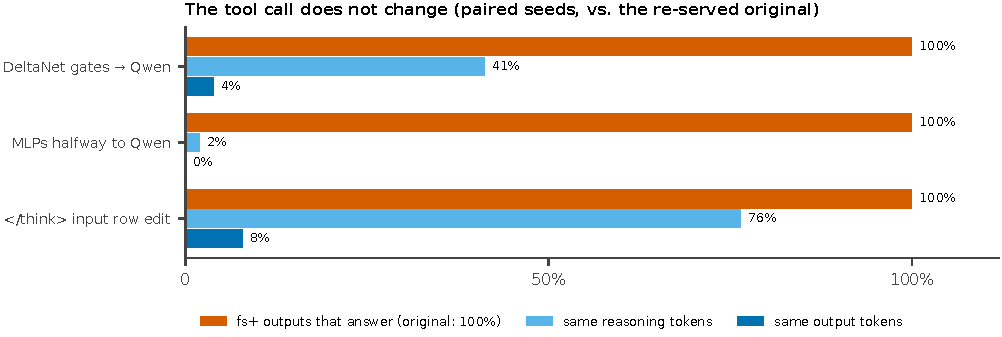
\includegraphics[width=\linewidth]{figs/attractor.pdf}
\caption{\textbf{The tool call does not change under three mechanism-level edits.} For three weight edits, share of false-completion outputs that still call \texttt{answer} (as the original does on all of them), and share of all 51 paired outputs whose reasoning, or whole output, is token-identical to the re-served original with the same seed. Six development contexts, 8 seeds each, plus three text prompts. Two runs of the unmodified model were not compared; H5, which leaves the reasoning weights unchanged unless \texttt{</think>} is in the prompt, gives a partial reference (\attHfivehalfGuiReason{} identical GUI reasoning prefixes).}
\label{fig:attractor}
\end{figure}
